\exercise{Motifs in a large network\label{exRGmotif}}{2}
In this chapter we derived the formula $n_{\rm motif} = z^k N^{n-k}/s$ for the approximate number of instances of a motif with 
$n$ nodes, $k$ links, and symmetry number $s$ in a network with $N$ nodes and mean degree $z$. Let's use this formula to estimate some motif counts in a network of $N=10.000$ nodes and $z=10$. 

\subquestion 
To build up some confidence in the formula, let's use it to estimate the number of nodes in the network (so the motif we are looking for is just a node.)

\solution
A motif consisting only of one node has $n=1$, $k=0$, $s=1$. Substituting into the formula gives us
\eq{
n_{\cdot} = \frac{1}{s} z^k N^{n-k} = N=10,000.
}
So, this worked out well. 

\subquestion 
Does the motif formula also yield the right result when we use it to compute the number of links?

\solution
Let's see: A link motif consists of two nodes ($n=2$) connected by one link $k=1$. There are two ways in which we can assign numbers 1,2 two two linked nodes such that the link connecting them is the same link ($s=2$). So our estimate for the number of links would be 
\eq{
n_{-}=\frac{1}{s} z^k N^{n-k} = \frac{z N}{2}
}
Indeed we know that $z=2K?N$ and hence 
\eq{
n_{-}=K
}
which makes sense.

\subquestion
Now, estimate the number of 4-cycles ($\square$).

\solution
A 4 cycle consists of $n=4$ nodes and $k=4$ links. 
Using our general motif formula
\eqa{
n_{\mbox{4-cycle}} &=& \frac{z^4}{s} (N-1)^{4-4} \\
&=& \frac{z^4}{s}
}
Now we have to find the symmetry number $s$. So, we find this number by asking how many different ways are there in which we can assign numbers (1,2,3,4) to the nodes in the four cycle such that we end up with exactly the same links. 

Suppose I want my 4-cycle to use the links (1,2), (2,3), (3,4), (4,1). We can think as follows: First we place the 1 into one of the nodes of the cycle. It can go into any of the 4 nodes. That is 4 choices. The 2 must be next to the 1, otherwise we are not using the (1,2) link. We can place the 2 clockwise or counter clockwise from the 1. That is 2 choices for the 2. The three must be next to the 2 so there is one spot left where it can go. The four then goes in the remaining spot, so no more choices for these numbers. 

So we have 4 choices for the 1 and 2 choices for the 2 multiplying these we get
\eq{
s=8
}
So the full formula is 
\eq{
n_{\mbox{4-cycle}} = \frac{z^4}{8}=
}
In case you still have doubts that the correct number is 8 here are 8 cycles that all use the same links,
\begin{center}
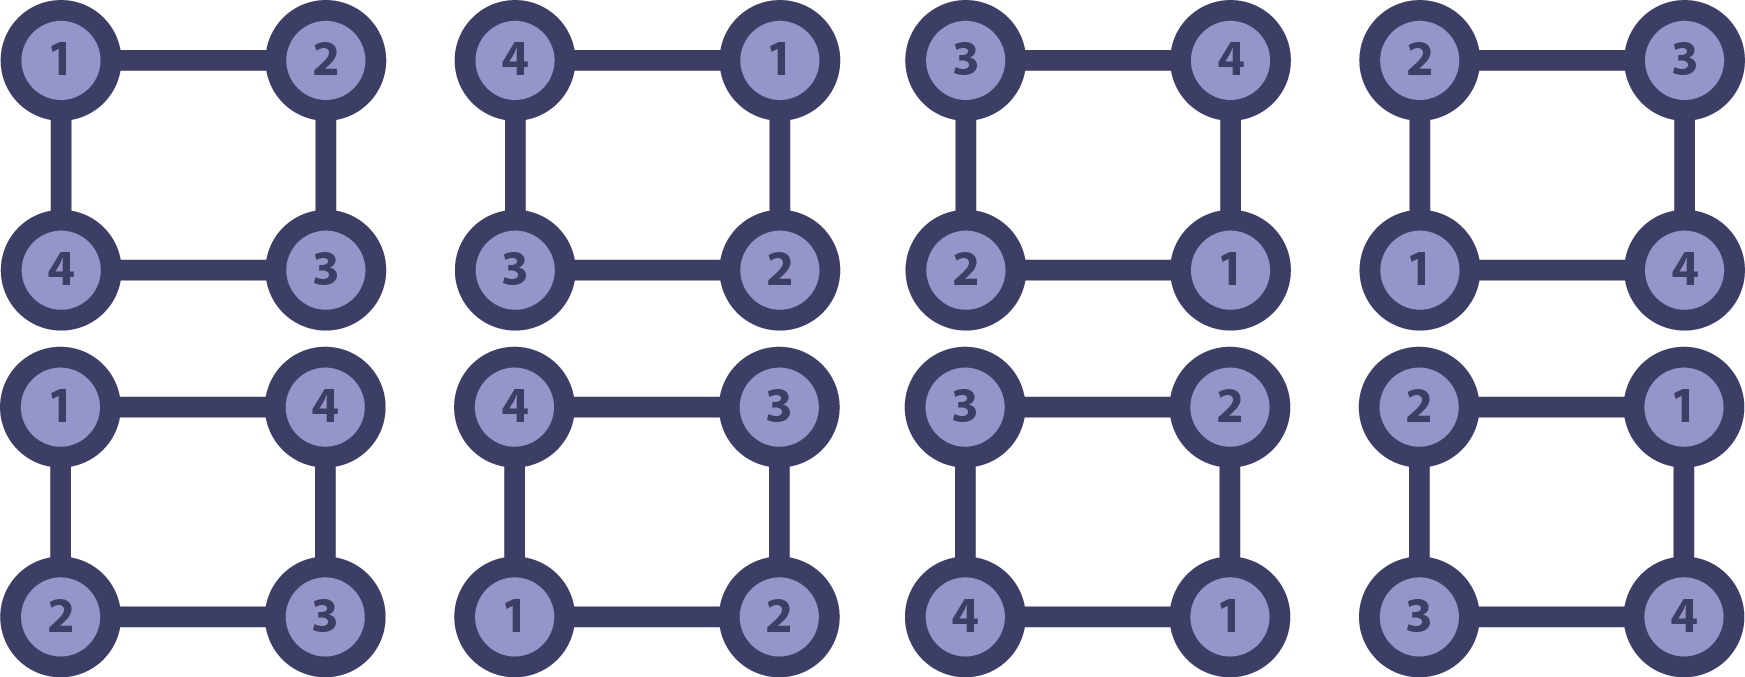
\includegraphics[width=0.6\textwidth]{cyclesymmetry}
\end{center}
Of course we can spot a pattern here. We can think of it as a four-fold rotational symmetry and a mirror symmetry that turns a clockwise cycle into a counter-clockwise cycle. From this observation we can conjecture that the symmetry number for any $n$-cycle is $s=2n$ which is indeed the case. 

Finally you may wonder if we can actually use the approximate formula in this case. For $N=100.000$ and $n=4$ the approximation we have made is 
\eq{
100000\cdot 99999 \cdot 99998 \cdot 99997 \approx 100000^4 
}
This is the same as saying 
\eq{
9.99940001099994\cdot{}10^{19} = 10^{20}
}
The approximate number is 99.994\% of the true value, which means the error is only $0.006\%$. For such large networks the approximation works pretty well.  